% !TEX root = main.tex
% Main text: abstract through conclusion. Two theorems (time separation; separation not from capacity),
% three lemmas and one proposition. General-K statements, constants and proofs are in the appendix.
\begin{abstract}
A Transformer can contain an exact program for counting the letters of a prompt, both one that writes only the
final count and one that writes every running count. Do intermediate steps help because they add labels, or because
they change which program gradient training reaches? We answer this for counting with $n$ hidden updates, where each
letter is the query with probability $p<1/2$ and $\lambda=1-2p$. The mechanism is simple: a feature that reads $k$
letters sees the final count only through a factor $\lambda^{n-k}$, while a displayed running count leaves a local
signal of variance $1-\lambda^2$. We prove two separations.
(1)~\emph{In time:} from the same small seed of a two-block Transformer, step training gives every transition a
positive margin in time polynomial in $n$, while outcome training stays near chance for time $\lambda^{-n}$.
(2)~\emph{Not from capacity:} in a model family that contains exact executors for both formats, from every seed in an
explicit open set, step training reaches positive margins on every transition, while outcome training converges to a
suboptimal minimum with accuracy $(1+\lambda^{n-1})/2$.
Experiments confirm the $\lambda^{-n}$ plateau and the trap, and show that the advantage survives matched label budgets
and learned attention routing.
\end{abstract}

% ===================================================================
\section{Introduction}
\label{sec:intro}

Training on intermediate steps makes many reasoning tasks learnable
\citep{nye2021scratchpads,wei2022cot,lightman2023verify}. Is that because steps give more labels, or because they
change which program gradient descent can reach? We answer this for the simplest task where the question is
non-trivial: counting how often a query letter occurs, modulo two.

The task has one parameter that controls everything. Each letter is the query letter with probability $p<1/2$; write
$\lambda=1-2p$. An outcome label is the parity of all $n$ letters, so a feature that reads only $k$ of them sees the
label through $n-k$ letters it never observed, and each unseen letter multiplies the correlation by $\lambda$
(\cref{fig:chain}). A step label is the next running count, which depends on one new letter only.

\paragraph{Contributions.} We prove that this difference decides what training reaches, in two theorems that each
compare the two formats from the same seed.

\begin{center}\small
\begin{tabular}{@{}p{0.34\linewidth}p{0.29\linewidth}p{0.29\linewidth}@{}}
\toprule
 & Step training & Outcome training\\
\midrule
\textbf{\Cref{thm:time}: separation in time} (two-block Transformer, same seed, same trained parameters) &
positive margins in time $\operatorname{poly}(n)$ & near chance for time $\lambda^{-n}$\\
\textbf{\Cref{thm:matched}: separation not from capacity} (one family containing both exact programs) &
positive margins on every transition & converges to a one-letter trap\\
\bottomrule
\end{tabular}
\end{center}

\Cref{thm:time} shows that outcome training is exponentially slower. Its trained family cannot express the outcome
program, so it leaves open that outcome training simply lacks capacity. \Cref{thm:matched} removes that explanation:
the failure comes from the loss, not from what the model can represent. Experiments test both theorems and show that
the advantage survives matched label budgets and learned attention routing (\cref{sec:experiments}).

\paragraph{Relation to \citet{kim2024parity}.} Kim and Suzuki prove that a Transformer learns parity with
teacher-forced chain of thought but not without it. Our setting differs in three ways. \emph{Task:} they
use worst-case $k$-parity, which is hard for any gradient method by a statistical-query argument;
counting with $p<1/2$ is a much easier target whose difficulty $\lambda$ can be tuned, so the fact that
outcome training still stalls points to the supervision format rather than the hardness of the task.
\emph{Architecture:} they use position-only attention, a fixed link function and one large gradient
step; we analyse a two-block Transformer for the plateau and gradient flow on readouts and query--key
strengths for the positive result. \emph{Kind of negative result:} theirs holds for every
algorithm with an approximate gradient oracle, which is stronger in form than our gradient-flow
plateau near small initialization. In exchange we obtain an explicit horizon dependence $\lambda^{-n}$,
and a same-family trap that rules out the explanation that outcome training merely lacks capacity.

% ===================================================================
\section{Setup}
\label{sec:setup}
\label{sec:setting}

\paragraph{Task.} A prompt has a start bit $s_0$, uniform on $\{0,1\}$, and letters $w_1,\ldots,w_n$ drawn
i.i.d.\ from an alphabet in which the query letter $w^\star$ has probability $p\in(0,1/2)$. With
$b_t=\mathbf 1[w_t=w^\star]$, the running count is
\[
 s_t=s_0+b_1+b_2+\cdots+b_t\pmod 2,\qquad t=1,\ldots,n .
\]
In sign form, put $S=(-1)^{s_0}$ and $C_t=(-1)^{b_t}$. Then
\begin{equation}
 (-1)^{s_n}=S\,C_1C_2\cdots C_n,\qquad \E[C_t]=1-2p=\lambda .
 \label{eq:tracking}
\end{equation}
So the answer is a product of signs, as in parity, but each sign is biased towards $+1$. The
\emph{contraction coefficient} $\lambda\in(0,1)$ is the only property of the task that enters our
bounds. For counting modulo $K$ the same role is played by the largest modulus of a nontrivial
Fourier coefficient of one letter, and the arguments below extend; we treat the binary case only.

\begin{figure}[t]
\centering
\resizebox{\linewidth}{!}{% Conceptual figure: counting modulo K as a cyclic chain, and what each supervision format sees.
\begin{tikzpicture}[>=Stealth, font=\small,
  state/.style={circle, draw=royalazure!80!black, fill=royalazure!12, minimum size=7mm, inner sep=0pt},
  tok/.style={rectangle, rounded corners=2pt, draw=black!45, fill=black!4, minimum width=7mm, minimum height=5.5mm, inner sep=1pt},
  sup/.style={rectangle, rounded corners=2pt, draw=royalazure!80!black, fill=royalazure!12, minimum width=7mm, minimum height=5.5mm, inner sep=1pt},
  hid/.style={rectangle, rounded corners=2pt, draw=black!30, dashed, fill=white, text=black!45, minimum width=7mm, minimum height=5.5mm, inner sep=1pt}]

% ---------------- (a) cyclic chain ----------------
\begin{scope}[shift={(0,0)}]
  \foreach \i/\lab in {0/0, 1/1, 2/2, 3/{K{-}1}} {
    \node[state] (c\i) at ({90-\i*90}:1.25) {$\lab$};
  }
  \foreach \i/\dir in {0/90, 1/0, 2/-90, 3/180} {
    \draw[->, black!55] (c\i) to[out=\dir+28, in=\dir-28, looseness=6] node[pos=0.5, font=\scriptsize, fill=white, inner sep=0.5pt] {$1{-}p$} (c\i);
  }
  \draw[->, thick, royalazure] (c0) to[bend left=22] node[font=\scriptsize, above right=-1pt] {$p$} (c1);
  \draw[->, thick, royalazure] (c1) to[bend left=22] node[font=\scriptsize, below right=-1pt] {$p$} (c2);
  \draw[->, thick, royalazure, dashed] (c2) to[bend left=22] node[font=\scriptsize, below left=-1pt] {$p$} (c3);
  \draw[->, thick, royalazure] (c3) to[bend left=22] node[font=\scriptsize, above left=-1pt] {$p$} (c0);
  \node[align=center, font=\footnotesize] at (0,-2.6)
    {$s_t=s_{t-1}+b_t\ (\mathrm{mod}\ K)$\\[2pt] $\mathbf T=(1-p)\,\mathbf I+p\,\mathbf R$};
  \node[font=\small\bfseries] at (-2.3,1.75) {(a)};
\end{scope}

% ---------------- (b) what each format supervises ----------------
\begin{scope}[shift={(3.4,0.95)}]
  \node[font=\small\bfseries] at (-0.35,0.8) {(b)};
  % outcome row
  \node[anchor=west, font=\footnotesize] at (0,0.8) {Outcome: supervise $s_n$ only};
  \node[tok] (o0) at (0.45,0) {$s_0$};
  \node[tok] (ow1) at (1.35,0) {$w_1$};
  \node[hid] (os1) at (2.25,0) {$s_1$};
  \node[tok] (ow2) at (3.15,0) {$w_2$};
  \node[hid] (os2) at (4.05,0) {$s_2$};
  \node at (4.85,0) {$\cdots$};
  \node[tok] (own) at (5.65,0) {$w_n$};
  \node[sup] (osn) at (6.55,0) {$s_n$};
  \draw[decorate, decoration={brace, amplitude=4pt, mirror}, black!60] (1.0,-0.42) -- (6.0,-0.42)
    node[midway, below=4pt, font=\footnotesize, align=center] {$n$ hidden letters: each Fourier mode contracts by $\le\mixrate$ per letter};
  % step row
  \node[anchor=west, font=\footnotesize] at (0,-1.75) {Step: supervise every $s_t$ from the displayed $s_{t-1}$};
  \node[tok] (p0) at (0.45,-2.55) {$s_0$};
  \node[tok] (pw1) at (1.35,-2.55) {$w_1$};
  \node[sup] (ps1) at (2.25,-2.55) {$s_1$};
  \node[tok] (pw2) at (3.15,-2.55) {$w_2$};
  \node[sup] (ps2) at (4.05,-2.55) {$s_2$};
  \node at (4.85,-2.55) {$\cdots$};
  \node[tok] (pwn) at (5.65,-2.55) {$w_n$};
  \node[sup] (psn) at (6.55,-2.55) {$s_n$};
  \draw[rounded corners=3pt, thick, lightmauve!80!black] (1.83,-2.95) rectangle (3.55,-2.15);
  \draw[->, thick, lightmauve!80!black] (3.55,-2.55) -- (ps2.west);
  \node[font=\footnotesize, align=center] at (3.5,-3.45) {one local transition $(s_{t-1},w_t)\mapsto s_t$: innovation $\ge1-\mixrate^2$};
\end{scope}
\end{tikzpicture}
}
\caption{\textbf{One counting process, two views of it.}
(a)~Counting is a two-state Markov chain: each letter keeps the count with probability $1-p$ and flips it with probability $p$.
(b)~Outcome supervision labels only $s_n$, so a feature that reads $k$ letters sees the label through
$n-k$ unseen steps, and its correlation shrinks like $\mixrate^{n-k}$ (\cref{thm:main}). Step supervision
displays the previous count and labels the next one, which keeps a rule signal of variance $1-\mixrate^2$
(\cref{sec:credit}).}
\label{fig:chain}
\end{figure}

\paragraph{Two formats.} Both formats see the same prompt. The \emph{outcome loss} $\Lout$ is the
cross-entropy of the final count $s_n$. The \emph{step loss} $\Lstep$ is the teacher-forced cross-entropy of
each transition: from a displayed count $s$ and the next letter $w$ to the next count $s'$, which is $s+1$ if $w=w^\star$
and $s$ otherwise (mod $2$), averaged over the positions $t\ge2$.

\paragraph{Model.} We use a Transformer with two causal attention/ReLU blocks, relative position
biases, no LayerNorm and a linear readout; $\bm\theta$ denotes all parameters.

\begin{proposition}[Both programs exist]
\label{prop:represent}
With widths linear in $n$, this architecture has parameters $\thstep$ and $\thout$ at which greedy decoding
is correct on every prompt, in the step and the outcome format respectively (\cref{app:architectures}).
\end{proposition}

\paragraph{Initialization.} Our results for the full Transformer use \emph{small initialization}: all weights at scale
$\varepsilon$ with zero readout, and MLP biases bounded away from zero so that the ReLU pattern is fixed
near the seed (\cref{ass:arch,ass:init}). At the executor widths of \cref{prop:represent}, which grow linearly in $n$, keeping
the ReLU pattern fixed needs $\varepsilon\le cn^{-1/2}$; this is why we assume $\varepsilon\le c\min(\lambda,n^{-1/2})$
(\cref{rem:end-width}). Small initialization is the standard regime for gradient-flow analysis of feature learning, and it
is where the plateau is visible; the experiments also leave it.
Throughout, $c,C>0$ are constants that depend on the architecture but not on $n$, $\varepsilon$ or $\lambda$;
they are listed in \cref{app:setup}.

% ===================================================================
\section{Why the two formats separate}
\label{sec:credit}
\label{sec:outcome}

We measure how much information about the label reaches a parameter update. Write the model's
output as one logit $z_{\bm\theta}$ (the difference of the two count logits) and fix the start bit.
The \emph{outcome credit} is $\|\nabla_{\bm\theta}\E[z_{\bm\theta}\,(-1)^{s_n}]\|$: the part of the outcome
gradient that depends on the answer (\cref{lem:gradient-split}).

\paragraph{Each unseen letter costs a factor $\lambda$.} Let a feature $h$ read only the letters in a set $A$. Averaging
over the other letters replaces each of their signs by its mean, so by \cref{eq:tracking}
\begin{equation}
 \E\bigl[(-1)^{s_n}\bigm| \text{letters in }A\bigr]=S\prod_{t\in A}C_t\cdot\lambda^{n-|A|},
 \qquad\text{hence}\qquad
 \bigl|\E[h\,(-1)^{s_n}]\bigr|\le\lambda^{n-|A|}\,\|h\|_{L^2}.
 \label{eq:credit-degree}
\end{equation}

\paragraph{The network reads few letters at a time.} Expand the network in powers of its attention scores.
With all scores zero, attention is uniform and each term reads at most one letter. We use only two facts
about this expansion (\cref{prop:score-degree}): apart from a letter-free part of size $C\varepsilon$, the terms of
order $k$ \emph{read at most $2k+1$ letters} and have \emph{total size at most $C\varepsilon^{2+4k}$}.

\begin{lemma}[Outcome credit vanishes]
\label{thm:main}
With the start bit fixed, \cref{eq:credit-degree} holds for every letter set $A$ and every feature $h$ of
those letters. If $\varepsilon\le c\min(\lambda,n^{-1/2})$, then near the seed
\[
 \bigl\|\nabla_{\bm\theta}\E[z_{\bm\theta}\,(-1)^{s_n}]\bigr\|\ \le\ C\,\varepsilon\,\lambda^{n}.
\]
\end{lemma}

\emph{Sketch of proof.} The letter-free part sees the answer only through its mean $S\lambda^n$, giving credit
$C\varepsilon\lambda^n$. An order-$k$ term reads at most $2k+1$ letters, so by \cref{eq:credit-degree} its credit is at most
$C\varepsilon^2\lambda^{n-1}(\varepsilon^4/\lambda^2)^k$, a geometric series bounded by $C\varepsilon\lambda^n$ (\cref{app:credit-proof}).

\paragraph{A displayed count leaves a local signal.} The displayed count alone predicts the next count with
probabilities $(1-p,p)$. Let $S$ and $C$ be the signs of the displayed count and the current letter. In sign form the
step label is $SC$, and its part not predicted by the displayed count is the \emph{rule signal} $S(C-\lambda)$, of variance
$1-\lambda^2$. It is paid once, for one letter, whereas an outcome label pays $\lambda$ for every unseen letter. The two
theorems below turn this difference in signal into a difference in what training reaches.

% ===================================================================
\section{Theorem 1: separation in time}
\label{sec:step}
\label{sec:time}

\paragraph{One formula for both theorems.} In both theorems the step prediction has the form
\begin{equation}
 f=S\bigl(a+g\tanh(qk)\,C\bigr),
 \label{eq:gate-logit}
\end{equation}
with a \emph{state readout} $a$ (trust the displayed count), a \emph{gate readout} $g$ (use the current letter) and a
\emph{gate strength} $qk$, a product of query and key scales. The step label is $SC$, so the step program needs
$g\tanh(qk)$ large; the outcome loss rewards it only through the weak factor of \cref{eq:binary-loss-mixture} below.
Step training grows $g\tanh(qk)$; the two theorems show that outcome training does not.

\paragraph{The seed.} In the two-block Transformer, the second block has a gate head that attends to the displayed count
and the current letter, and its output reaches the logits through a count readout and a gate readout. With all other
maps fixed, the step logit reduces exactly to \cref{eq:gate-logit} (\cref{lem:J-reduce}). Both readouts start at zero, the
query and key scales start at size $\varepsilon$, and gradient flow trains the two readouts and the two scales. The seed is
\emph{aligned} if its initial gate already points the right way ($q_0k_0<0$ in \cref{app:step-supplied-routing}); a random choice
of the two signs is aligned with probability $\frac12$.

\begin{theorem}[Separation in time]
\label{thm:time}
Start the two-block Transformer, with widths at most linear in $n$, from an aligned seed with $\varepsilon\le c\min(\lambda,n^{-1/2})$,
and train the same parameters under each loss.
\begin{thmparts}
\item\label{thm:joint} \emph{Step training learns.} Every transition has positive margin for all $t\ge T_{\mathrm{step}}$, and $\Lstep\to0$, where
\[
 T_{\mathrm{step}}\le\frac{C_p}{\varepsilon^4}\,\sqrt{d}\,\log\frac{d}{\varepsilon},
\]
with $d$ the head width and $C_p$ depending only on $p$. At executor width ($d\asymp n$,
$\varepsilon\asymp n^{-1/2}$) this is $O(n^{5/2}\log n)$.
\item\label{thm:outcome-end} \emph{Outcome training stalls.} For all $t\le c\lambda^{-n}$,
\[
 \Lout(\bm\theta(t))\ \ge\ \log2-C\varepsilon^2\lambda^n
 \qquad\text{and}\qquad
 \Pr\nolimits_{\bm\theta(t)}(\text{correct answer})\ \le\ \tfrac12+C\varepsilon\lambda^{n/2}.
\]
This part holds for every small seed of \cref{ass:init}, even if every parameter of the Transformer is trained.
\end{thmparts}
\end{theorem}

\emph{Sketch of (ii).} Along gradient flow, $\frac{d}{dt}\Lout=-\|\nabla\Lout\|^2$, so by Cauchy--Schwarz
$\|\bm\theta(t)-\bm\theta_0\|^2\le t\,(\Lout(\bm\theta_0)-\Lout(\bm\theta(t)))$. Near the seed, \cref{thm:main} implies the loss can fall
by at most $C\varepsilon^2\lambda^n$, so the flow travels at most $\sqrt{t\,C\varepsilon^2\lambda^n}$, which is smaller than the
neighbourhood until $t$ is of order $\lambda^{-n}$ (\cref{app:end}). The seed above satisfies \cref{ass:init}
(\cref{cor:joint-outcome}), so both parts start from the same point.

\emph{Sketch of (i): why joint training succeeds.} The flow reduces exactly to the three numbers $a$, $g$, $qk$ of
\cref{eq:gate-logit} (\cref{lem:J-reduce}). The count prior first gives $g$ a direction, and the gradient of $qk$ is proportional to
$g$, which keeps an aligned gate aligned. A monotone balance between $g$ and $a$ then holds
$g$ above a fixed floor (\cref{lem:J-align,lem:J-floor}), $|qk|$ grows exponentially to order one, and a gradient lower bound
proportional to $\tanh^2(qk)$ gives positive margins after time $O(\varepsilon^{-4}\log\frac1\varepsilon)$ (\cref{lem:J-grow}). Measured solve
times scale as $\varepsilon^{-4.0}$ to $\varepsilon^{-4.3}$, also from misaligned seeds, which first turn around (\cref{tab:J-ode}).

% ===================================================================
\section{Theorem 2: the separation is not from capacity}
\label{sec:matched}
\label{sec:two-path-trap}

The trained family of \cref{thm:time} cannot express the outcome program, so a reader may suspect that outcome training
fails for lack of capacity. We now fix one family that contains \emph{both} exact executors. The next identity shows where
outcome training will be caught.

\begin{lemma}[One-letter loss identity]
\label{lem:binary-loss-mixture}
For any predictor that reads only the start bit and the last letter, with $L_{\mathrm{sym}}$ the loss with random labels,
\begin{equation}
 L_{\mathrm{out}}=L_{\mathrm{sym}}+\lambda^{n-1}\bigl(L_{\mathrm{step}}-L_{\mathrm{sym}}\bigr).
 \label{eq:binary-loss-mixture}
\end{equation}
\end{lemma}
\emph{Proof.} The hidden product $\prod_{t<n}C_t$ is independent of the inputs and equals $\pm1$ with probability
$(1\pm\lambda^{n-1})/2$; condition on it (\cref{app:contraction}). \hfill$\square$

So the outcome loss is a $\lambda^{n-1}$-weak copy of the step loss. Its minimizer is a confident one-letter guess that is
right with probability only $(1+\lambda^{n-1})/2$. Gradient flow is captured by exactly this guess.

\paragraph{The family.} Routing is supplied: at transition $t$ the model sees the previous count, the current letter
and the mean $u$ of the first $t$ bits; at the answer it sees $s_0$, the last letter and the mean of all bits. Writing $S$
and $C$ for the signs of the displayed count and the current letter,
\begin{equation}
 f(S,C,u)=\underbrace{S\bigl(a+g\tanh(qk)\,C\bigr)}_{\text{gate path, as in \cref{eq:gate-logit}}}
 \;+\;\underbrace{h_\phi(u,S)}_{\text{averaging path}},
 \label{eq:two-path-model}
\end{equation}
with all parameters trained. The averaging path is a one-hidden-layer ReLU network $h_\phi(u,S)=\sum_iv_i\relu(w_iu+d_iS+b_i)$
with $6(n+1)$ units, and $\phi=(v_i,w_i,d_i,b_i)_i$. Here $\tanh$ is the hyperbolic tangent, a rescaled sigmoid $\sigmoid$:
\[
 \tanh(x)=\frac{e^{x}-e^{-x}}{e^{x}+e^{-x}}=2\sigmoid(2x)-1\in(-1,1),\qquad \sigmoid(x)=\frac1{1+e^{-x}} .
\]
The gate path executes the step program; the averaging path can read the full count and executes the outcome program
(\cref{prop:two-path-trap}). The experiments show that step training can also learn this routing (\cref{tab:reach}).

\begin{theorem}[The separation is not from capacity]
\label{thm:matched}
For each $n$ there is an explicit set $\mathcal U_n$ of seeds, open among seeds with zero readouts ($a=g=v=0$) and
nonempty for $n\ge n_0(p)$, such that from every seed in $\mathcal U_n$:
\begin{thmparts}
\item \emph{Step training learns:} after a time $O\bigl(p^{-2}\log(1/p)\,/\tanh^2(q_0k_0)\bigr)$, every transition has margin
at least $1/2$, at all later times.
\item \emph{Outcome training is trapped:} it converges to a local minimum with logits $\log\frac{1+\lambda^{n-1}}{1-\lambda^{n-1}}\,SC$, its loss
never falls below the loss of that minimum, and its accuracy tends to
\[
 \frac{1+\lambda^{n-1}}2\ <\ 1 .
\]
\end{thmparts}
\end{theorem}

\begin{figure}[t]
\centering
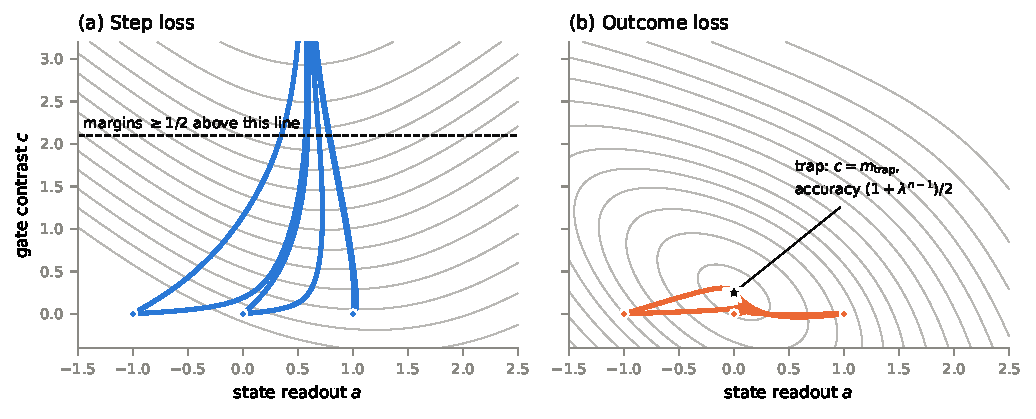
\includegraphics[width=\linewidth]{figures/two_path_phase.pdf}
\caption{\textbf{The same seeds, two losses.} Gradient flow of the two-path family (curves; dots are starting points),
shown in the plane of the state readout $a$ and the gate contrast $g\tanh(qk)$, over level sets of the loss (gray).
(a)~Under the step loss the contrast grows without bound and the margins become positive.
(b)~Under the outcome loss every trajectory converges to the one-letter trap (star). Here $n=4$, so that the
trap is visible; for larger $n$ it moves towards the origin.}
\label{fig:two-path-phase}
\end{figure}

The seeds live in the reduced family and are not at small scale: the gate starts at order one while the averaging
path starts small. $\mathcal U_n$ contains, for example, the seed $q_0=k_0=1$ with two active ReLUs of size about
$p/\sqrt{n\log(1/p)}$ and an averaging path that ignores $S$, together with every small enough perturbation of it
(\cref{lem:seed-set}); $n_0(1/4)=32$. The exact conditions are in \cref{app:matched-proof}.

\emph{Sketch of proof.} \emph{Outcome half.} At zero readout the loss is $\log2$, only $O(\lambda^{2(n-1)})$ above the trap.
Gradient flow turns a small loss gap into a short path, so the flow cannot leave the region where each ReLU keeps its
sign. There the loss is a strictly convex function of four effective coefficients, and its only minimizer is the trap
(\cref{app:random-trap-certificate}). \emph{Step half.} In the same region the averaging path is affine in $(u,S)$, so the step logit is
\cref{eq:gate-logit} plus a small affine term. (a)~\emph{The gate grows:} $g\tanh(qk)$ increases at rate at least $\tanh^2(q_0k_0)$ times
the current error rate.
(b)~\emph{The state readout is bounded:} $a$ stays in $[0,\log\frac{1-p}p]$ up to small corrections.
(c)~\emph{The averaging path stays small:} $h_\phi$ is driven only through its dependence on $S$, at a rate set by
$\dot a$; since $a$ stays in a fixed interval, a conservation law keeps $h_\phi$ within a factor $O(1/p)$ of its initial size, so
it never competes with the gate.
(d)~\emph{Margins persist:} once the loss is below the smallest cell probability, no margin can turn negative again
(\cref{app:matched-proof}).

The outcome executor is in the family at zero loss, and the same gate path that outcome training leaves weak is driven to
a margin by step training. With initialization, architecture and expressivity all matched, only the loss differs.

% ===================================================================
\suppressfloats[t]
\section{Experiments}
\label{sec:experiments}
\label{sec:validation}

We test both theorems with binary counting at $p=1/4$ ($\lambda=1/2$); protocols are in \cref{app:experiments}.

\begin{figure}[t]
\centering
\resizebox{\linewidth}{!}{%% Experiments figure: (a) from overview.tex, (b,c) from theory_measurement.tex (same data sources).
\definecolor{stepc}{HTML}{0072B2}\definecolor{outc}{HTML}{D55E00}\definecolor{theoc}{HTML}{009E73}
\definecolor{mutedc}{HTML}{6E6E6E}\definecolor{errc}{HTML}{EDB79C}
\begin{tikzpicture}
\pgfplotsset{every axis/.style={width=0.4\linewidth, height=4.9cm, axis line style={black!80}, tick style={black!80},
  tick label style={font=\footnotesize}, label style={font=\small}, title style={font=\small, at={(0,1)}, anchor=south west, xshift=-2pt},
  axis x line*=bottom, axis y line*=left}, every axis plot/.append style={line width=1pt}}
\begin{axis}[name=pa, title={\textbf{(a)} Training, $n=16$}, xlabel={Updates (thousands)}, ylabel={Exact accuracy (\%)},
  xmin=0, xmax=8, ymin=0, ymax=112, xtick={0,4,8}, ytick={0,50,100}, axis x line*=bottom, axis y line*=left, clip=false]
  \addplot[draw=none, fill=stepc, fill opacity=0.18, forget plot] coordinates {(1,0.55) (2,0.73) (3,0.82) (4,1.25) (5,9.77) (6,29.75) (7,49.33) (8,98.40) (8,100.00) (7,100.00) (6,100.00) (5,92.03) (4,1.90) (3,1.40) (2,1.35) (1,1.35)};
  \addplot[draw=none, fill=outc, fill opacity=0.18, forget plot] coordinates {(1,49.52) (2,49.73) (3,49.05) (4,48.92) (5,49.35) (6,49.92) (7,48.97) (8,49.15) (8,50.70) (7,50.70) (6,51.20) (5,51.08) (4,50.60) (3,50.70) (2,51.08) (1,51.08)};
  \addplot[theoc, dashed, line width=0.9pt, domain=0:8, samples=2] {100};
  \addplot[mutedc, densely dashed, line width=0.8pt, domain=0:8, samples=2] {50};
  \addplot[stepc, mark=square*, mark size=1.8pt] coordinates {(1,1.00) (2,1.05) (3,1.30) (4,1.45) (5,21.65) (6,73.40) (7,95.40) (8,100.00)};
  \addplot[outc, mark=*, mark size=1.9pt] coordinates {(1,50.40) (2,50.60) (3,50.40) (4,49.85) (5,50.25) (6,50.60) (7,50.25) (8,50.40)};
  \node[anchor=south west, font=\footnotesize, text=theoc, inner sep=1pt] at (axis cs:0.15,101.5) {Exact executor};
  \node[anchor=west, font=\small\bfseries, text=stepc] at (axis cs:0.2,86) {Step};
  \node[anchor=west, font=\scriptsize, text=stepc] at (axis cs:0.2,76) {8/10 seeds solve};
  \node[anchor=south west, font=\small\bfseries, text=outc, inner sep=1pt] at (axis cs:0.15,54) {Outcome};
  \node[anchor=north west, font=\scriptsize, text=mutedc, inner sep=1pt] at (axis cs:0.15,46) {Chance};
\end{axis}
\begin{semilogyaxis}[name=pb, at={(pa.east)}, anchor=west, xshift=1.6cm, title={\textbf{(b)} Plateau duration}, xlabel={Horizon $n$}, ylabel={Displacement time $\tau(0.1)$},
  xmin=3.6, xmax=14.4, xtick={4,8,14}, ymin=3, ymax=1e8, ytick={1e1,1e3,1e5,1e7}, ymajorgrids, major grid style={black!12}]
  \addplot[draw=none, fill=outc, fill opacity=0.18, forget plot] coordinates {(4,10638.7) (6,53401.7) (8,257804) (10,1.17632e+06) (12,5.46642e+06) (14,2.47378e+07) (14,3.29507e+07) (12,6.99489e+06) (10,1.54461e+06) (8,332934) (6,68528) (4,13708.5)};
  \addplot[draw=none, fill=stepc, fill opacity=0.18, forget plot] coordinates {(4,4.2576) (6,4.25798) (8,4.25824) (10,4.25841) (12,4.25855) (14,4.25866) (14,4.94345) (12,4.94354) (10,4.94365) (8,4.9438) (6,4.94399) (4,4.9443)};
  \addplot[outc, mark=*, mark size=1.8pt] coordinates {(4,12013.4) (6,60575.1) (8,290310) (10,1.30468e+06) (12,6.1887e+06) (14,2.74812e+07)};
  \addplot[stepc, mark=square*, mark size=1.7pt] coordinates {(4,4.33272) (6,4.3327) (8,4.33268) (10,4.33266) (12,4.33266) (14,4.33265)};
  \addplot[theoc, dashed, line width=0.9pt] coordinates {(4,12013.4) (6,48053.5) (8,192214) (10,768856) (12,3.07542e+06) (14,1.23017e+07)};
  \node[anchor=west, font=\footnotesize, text=outc] at (axis cs:4,4e6) {Outcome};
  \node[anchor=north east, font=\footnotesize, text=theoc] at (axis cs:14,1.538e+06) {$\mixrate^{-n}$};
  \node[anchor=south, font=\footnotesize, text=stepc] at (axis cs:10,13) {Step};
\end{semilogyaxis}
\begin{semilogxaxis}[name=pc, at={(pb.east)}, anchor=west, xshift=1.75cm, title={\textbf{(c)} Outcome accuracy follows $\mixrate^n$},
  xlabel={Remaining bias $\mixrate^n$}, ylabel={Outcome accuracy (\%)}, xmin=1e-5, xmax=0.8, xtick={1e-5,1e-3,1e-1},
  ymin=0, ymax=103, ytick={0,50,100}, ymajorgrids, major grid style={black!12}]
  \addplot[mutedc, densely dashed, line width=0.8pt, domain=1e-5:0.8, samples=2] {50};
  \addplot[theoc, dashed, line width=1pt, domain=1e-5:0.7, samples=120] {50*(1+x)};
  \addplot[only marks, outc, mark=*, mark size=1.6pt, error bars/.cd, y dir=both, y explicit, error bar style={errc, line width=0.8pt},
    error mark=none] coordinates {(0.015625,49.6) += (0,0.1) -= (0,0.1) (0.0877915,57.33) += (0,2.467) -= (0,1.633) (0.262144,70.33) += (0,5.667) -= (0,6.233) (0.531441,79.03) += (0,2.167) -= (0,1.933) (0.00390625,51.17) += (0,3.833) -= (0,2.367) (0.0390184,51.27) += (0,1.833) -= (0,2.167) (0.167772,61.73) += (0,3.967) -= (0,3.233) (0.430467,70.93) += (0,0.6667) -= (0,0.5333) (0.000976562,50.07) += (0,0.3333) -= (0,0.5667) (0.0173415,50.57) += (0,0.4333) -= (0,0.8667) (0.107374,55.37) += (0,1.233) -= (0,0.9667) (0.348678,71.13) += (0,2.667) -= (0,2.233) (0.000244141,50.37) += (0,0.5333) -= (0,0.9667) (0.00770735,51.93) += (0,1.467) -= (0,1.433) (0.0687195,51.53) += (0,4.367) -= (0,2.833) (0.28243,64.4) += (0,1.7) -= (0,1.7) (1.52588e-05,50.4) += (0,1.2) -= (0,1.1) (0.00152244,50.2) += (0,1) -= (0,1.3) (0.0281475,50.47) += (0,2.233) -= (0,2.967) (0.185302,57.23) += (0,1.867) -= (0,2.733)};
  \node[anchor=north west, font=\footnotesize] at (rel axis cs:0.03,0.98) {Spearman $\rho=0.91$};
  \node[anchor=north west, font=\footnotesize, text=theoc] at (rel axis cs:0.03,0.8) {State-only prior};
  \node[anchor=north west, font=\scriptsize, text=mutedc] at (rel axis cs:0.03,0.46) {Chance};
\end{semilogxaxis}
\end{tikzpicture}
}
\caption{\textbf{Outcome training stalls on an exponential plateau; step training does not.}
(a)~Full Transformer, $n=16$, zero readout, AdamW: median exact continuation accuracy and interquartile band over ten
paired seeds. Both formats admit an exact executor (\cref{prop:represent}).
(b)~Small initialization ($\varepsilon=0.002$): time for training to move a fixed distance from the seed, median and
interquartile band over three draws; the dashed guide is $\lambda^{-n}$ (\cref{thm:outcome-end}).
(c)~Outcome accuracy after $8$k updates in $20$ horizon--alphabet cells (means and seed ranges) against $\lambda^n$;
the dashed curve is the accuracy $\frac{1+\lambda^n}2$ of the state-only prior.}
\label{fig:experiments}
\end{figure}

\paragraph{Does \cref{thm:time} hold, and beyond its assumptions?} In the small-initialization regime the time to leave
the seed grows from $10^4$ at $n=4$ to $3\times10^7$ at $n=14$, at least as fast as $\lambda^{-n}$, while the step exit time
stays at $4.3$ for every $n$, and no ReLU changes sign (\cref{fig:experiments}b). Outside the theorem, a full Transformer
trained with AdamW at $n=16$ solves $8$ of $10$ seeds with steps while outcome training stays at chance
(\cref{fig:experiments}a). Across horizons and alphabets, outcome training learns the state-only prior
$\frac{1+\lambda^n}2$ (Spearman $\rho=0.91$) and essentially nothing beyond it (median excess $0.2$ points,
\cref{fig:experiments}c).

\paragraph{Does \cref{thm:matched} hold?} We run population gradient descent (step sizes $1$, $\tfrac12$ and $\tfrac14$, giving the
same results) in the two-path family from $12$ seeds that satisfy every condition of $\mathcal U_n$, checked numerically, at
$n\in\{36,40,48,64\}$: perturbations of the explicit seed with nonzero state weights on all units. Every transition
reaches margin $1/2$ by flow time $5$, far inside the theorem's upper bound ($T\approx265$ for these seeds); outcome
training ends after flow time $2\times10^4$ at exactly the one-letter accuracy $(1+\lambda^{n-1})/2$, with no ReLU changing
sign. Away from these seeds (Appendix, \cref{fig:two-path-sweep}), outcome training never escapes at $n=17$, and escapes
at $n=6,8$ only when ReLU kinks start inside the input range: this is the initialization boundary of the trap.

\paragraph{Is it just more labels, or supplied routing?} \input{sections/label_budget_result} Routing need not be
supplied either: training query--key maps, relative biases and readout together from a random initialization solves $16$
of $17$ step runs (the last reaches $99.95\%$), while matched outcome runs solve none within $300$k updates
(\cref{tab:reach}).

\begin{table}[t]
\caption{\textbf{Step training learns the routing; outcome training under the same protocol does not.}
Scores, relative bias and readout are trained by full-batch gradient descent from $\varepsilon=0.3$, with the same seeds for both
formats. Solved: every held-out prediction correct.}
\label{tab:reach}
\centering\small
\begin{tabular}{@{}rcccc@{}}
\toprule
 & \multicolumn{2}{c}{Step} & \multicolumn{2}{c}{Outcome (300k updates)}\\
\cmidrule(lr){2-3}\cmidrule(l){4-5}
$n$ & Solved & Updates to solve, median (range) & Solved & Answer accuracy (\%)\\
\midrule
6  & 5/5 & 44k (41--78k)   & 0/5 & 50--94\\
8  & 5/5 & 61k (46--99k)   & 0/5 & 50--55\\
12 & 4/5 & 77k (42--103k)  & 0/5 & 50\\
16 & 2/2 & 237k (208--266k) & 0/2 & 50--51\\
\bottomrule
\end{tabular}
\end{table}

% ===================================================================
\section{Related work and limitations}
\label{sec:related}
\label{sec:conclusion}

\paragraph{Related work.} Intermediate supervision has been studied through decomposition, locality,
expressivity and sample complexity
\citep{wies2023subtask,prystawski2023think,abbe2024globality,feng2023towards,merrill2024expressive,malach2023autoregressive,hanneke2026samplecomplexityautoregressivereasoning,wen2024sparse};
we fix the target and architecture and follow the gradient instead. Our credit bound is in the spirit of
failures of gradient learning for orthogonal targets \citep{shalevshwartz2017failures} and of
initialization-dependent parity learning \citep{abbe2025parities}, and is related to staircase and low-degree
analyses \citep{abbe2021staircase,abbe2023sgd,panigrahi2025progressive}; the new ingredient is a Transformer score
expansion that bounds how many letters each term reads. \citet{makkuva2025attention,makkuva2024local}
characterize good and bad minima of single-layer Transformers on Markov chains. \Citet{kim2024parity} are
discussed in \cref{sec:intro}. Counting is a cyclic automaton whose shallow shortcuts exist
\citep{liu2023automata}; we show that existence does not mean training finds them.

\paragraph{Limitations.} The full-Transformer results hold near small initialization; outside it we have experiments,
and one counterexample: for counting modulo $3$ at $n=8$, where $\lambda^{-8}\approx27$ is modest, two of three AdamW
outcome runs solve the task. \Cref{thm:joint} trains readouts and query--key strengths with routing
supplied; learned routing is only measured (\cref{tab:reach}). We treat binary counting; the contraction argument extends
to counting modulo $K$ with $\lambda$ the largest nontrivial Fourier modulus of one letter. \Cref{thm:matched} supplies routing and averaging and needs
$n\ge n_0(p)$; its seed conditions are sufficient, not necessary. Learning routing and unrestricted features jointly from
random weights remains open.
